% Manuscript source for a concise report of the central results. The letter
% leads with the positive empirical/model comparison and states explicitly
% which finer crossover claim remains unresolved.
\documentclass[aps,prl,twocolumn,superscriptaddress,floatfix,nofootinbib]{revtex4-2}

\usepackage{amsmath,amssymb,bm}
\usepackage{graphicx}
\usepackage[colorlinks=true,allcolors=blue]{hyperref}

\newcommand{\eps}{\varepsilon}
\newcommand{\avg}[1]{\left\langle #1 \right\rangle}
\newcommand{\Var}{\mathrm{Var}}

\begin{document}

\title{Counting statistics of signed order flow:\\
bunching beyond free transport and a memory-fixed variance exponent}

\author{Nelson Bol\'{\i}var}
\affiliation{Escuela de F\'isica, Facultad de Ciencias, Universidad Central de Venezuela, Caracas 1041-A, Venezuela}
\affiliation{Astrum Drive Technologies, 13024 Dallas Pkwy Unit 120 B, Frisco, TX 75034, USA}
\author{Gabriel Abell\'an}
\affiliation{Escuela de F\'isica, Facultad de Ciencias, Universidad Central de Venezuela, Caracas 1041-A, Venezuela}
\affiliation{Astrum Drive Technologies, 13024 Dallas Pkwy Unit 120 B, Frisco, TX 75034, USA}
\author{David Verrilli}
\affiliation{Escuela de F\'isica, Facultad de Ciencias, Universidad Central de Venezuela, Caracas 1041-A, Venezuela}

\date{\today}

\begin{abstract}
Reading the signed order flow of a market as the current of an open conductor
makes its full counting statistics measurable. We find the transferred flow to
be strongly bunched --- Fano factor of order $10^{3}$, growing with the counting
window, with superdiffusive variance --- which no free-fermion counting problem
can produce, since Pauli statistics bound the Fano factor below unity and give
diffusive growth. We confirm this against an explicit nonequilibrium Green
function calculation, which yields $\mathcal{F}=0.33$ and a variance exponent of
$0.99$. We then derive and confirm a parameter-free prediction: because a
correlation decaying as $\tau^{-a}$ produces a counting variance growing as
$T^{2-a}$, the two-component memory kernel measured in the correlation sector
fixes the counting exponent to the band $[1.00,1.83]$ with no free parameters.
The measured exponent falls inside it and exceeds unity in every asset under
four independent estimators, three of them constructed to be blind to a
drifting mean --- a confounder we show can imitate the finer prediction of a
drift \emph{within} that band, which we therefore report as consistent with the
data rather than established by it. Underlying both
results is
a structural observation that we believe corrects a growing literature: the
linear fluctuation symmetry $s(Q)=[2\avg{Q}/\Var(Q)]\,Q$, which this and related
systems display and which is naturally read as a fluctuation theorem, is an
algebraic identity satisfied by any Gaussian variable. The physical content of
market counting statistics lies entirely in the departures from it.
\end{abstract}

\maketitle

\paragraph*{Introduction.}
A market has two sides, and the net signed flow of executed orders between them
is a current: it counts something transferred, it fluctuates, and it responds to
what drives it. This reading makes available a measurement programme built for
transport in open, driven systems, whose most informative layer is the full
counting statistics of the charge transferred in a finite window
\cite{levitov1993,levitov1996,blanter2000,esposito2009}. Moments of the signed
flow accumulated over a window have been measured before, and their anomalous
scaling with window length attributed to order splitting \cite{maitrier2026};
what has not been carried over is the counting framework itself --- the
normalisation of the noise to its Poisson value through an effective transfer
quantum, and the reading of the log-ratio slope as an affinity conjugate to a
current.

There is a reason to be careful in doing so. Statistical-physics readings of
markets have proliferated: effective temperatures have been defined from return
ratios \cite{ramezani2025}, from order-book energies \cite{li2024entropy}, and
from holding-time asymmetries \cite{gao2026}, and a fluctuation--dissipation
relation has been reported for an effective Brownian particle in the book
\cite{yura2014}. Several of these rest on observing a log-ratio of forward and
reversed distributions that is linear in the observable. We show first that this
linearity, by itself, establishes nothing --- and then use that fact to isolate
what does.

\paragraph*{Setup.}
We use hourly and four-hourly candles for four cryptocurrency pairs over four
years --- eight series, with $3.5\times10^{4}$ hourly observations per asset.
Public candle data carry the taker-side volume, so the signed flow $\eps_t$
follows directly and no proprietary feed is required; continuous trading avoids
overnight gaps in the two-time estimates. Figures and quoted exponents are for
the hourly series unless stated otherwise.
Let $Q_T=\sum_{t=1}^{T}\eps_t$ be the flow transferred in a window of $T$
candles, and
\begin{equation}
  s(Q)=\ln\frac{P(Q_T=+Q)}{P(Q_T=-Q)}
\end{equation}
its fluctuation symmetry function. Analysis code and all logs are available
\cite{code_keldysh_finance}; the measurement and the model are developed at
length in companion papers \cite{paper1,paper2}.

\paragraph*{The identity.}
For a Gaussian $Q_T$ with mean $m_T$ and variance $V_T$,
\begin{equation}
  s(Q)=\frac{(Q+m_T)^2-(Q-m_T)^2}{2V_T}=\frac{2m_T}{V_T}\,Q ,
  \label{eq:identity}
\end{equation}
exactly and always. Writing the cumulant generating function
$F_T(\chi)=\ln\avg{e^{\chi Q_T}}=\chi m_T+\tfrac12\chi^2V_T$ and substituting
$\chi\to-A_T-\chi$ with $A_T=2m_T/V_T$ returns $F_T(\chi)$ identically, so the
Gallavotti--Cohen symmetry \cite{gallavotti1995,lebowitz1999} is satisfied as
well.

The consequence is worth stating without hedging. \emph{A measured linear
fluctuation symmetry whose slope equals $2\avg{Q}/\Var(Q)$ is not evidence of a
nontrivial fluctuation theorem.} It confirms that the estimator agrees with the
first two moments, and nothing more. In our data the measured affinity tracks
$2\avg{Q_T}/\Var(Q_T)$ across all windows and assets, and the cubic coefficient
of $s(Q)$ is consistent with zero where the data have power to resolve it
($c_3=0.024\pm0.119$ for one series at $T=16$) --- which is exactly what
Eq.~\eqref{eq:identity} demands and therefore carries no information about the
market.

This is a negative result, but it is the load-bearing one: it tells us that
anything informative must be sought in departures from Gaussianity, and it tells
us where to look.

\paragraph*{Bunching beyond free transport.}
The first departure is large. Because the carriers here are trades with a broad
size distribution, the Fano factor must be referred to the Poisson expectation
for carriers of the typical size rather than to the net transferred charge:
\begin{equation}
  \mathcal{F}(T)=\frac{\Var(Q_T)}{\bar q^{\,2}\,\avg{N_T}} ,
  \label{eq:fano}
\end{equation}
with $\bar q$ the median traded volume per trade --- the effective transfer
quantum --- and $N_T$ the number of trades in the window. A Poisson stream of
$N_T$ independent transfers of size $\pm\bar q$ gives $\mathcal{F}=1$
identically, so Eq.~\eqref{eq:fano} is the noise-to-Poisson ratio and is
directly comparable with the device value below. Measured at $T=1$ it ranges
from $905$ to $3342$ across the eight series studied, and grows as $T^{0.19}$
to $T^{0.28}$ [Fig.~\ref{fig:fano}]. The counting variance grows
superdiffusively, with log-slopes of $1.22$ to $1.37$ --- and $1.10$ to $1.36$
under the drift-blind estimators introduced below, so the excess over unity
does not rest on the mean --- against $[0.90,1.14]$ for a permutation null that
preserves the marginal distribution while destroying memory.

To fix what this excludes, we computed the same quantities for an explicit
transport device: a single level between two biased leads with a structured
hybridisation, evolved through a bias quench with nonequilibrium Green functions
\cite{jauho1994} and counted with the standard construction
\cite{levitov1996,schoenhammer2007}. Numerical controls bound the calculation
--- unitarity to $8\times10^{-16}$, and agreement between the zero-frequency
noise and the second counting cumulant, computed by independent routes, to
$1.3\times10^{-9}$. The device returns $\mathcal{F}=0.332$--$0.341$ and a
variance exponent running from $0.94$ to $0.99$.

The gap is three to four orders of magnitude in level and qualitative in growth,
and it cannot be closed by tuning. Sub-Poissonian noise is the Pauli
antibunching of free fermions and is bounded above by unity for any coupling,
bias or temperature; diffusive growth is what finite-memory single-channel
transport gives at long times. Because these are bounds on statistics rather
than on parameters, the measured values require two separable ingredients: a
heavy-tailed distribution of transfer sizes for the level, since a compound
process gives $\mathcal{F}\sim\avg{q^2}/\bar q^{2}$, and genuine long memory for
the growth. This places the missing physics in the interaction between order
flow and available liquidity, which is where the microscopic account of
order splitting puts it \cite{lillo2005,sato2023prl,sato2023prr}.

\begin{figure}[t]
  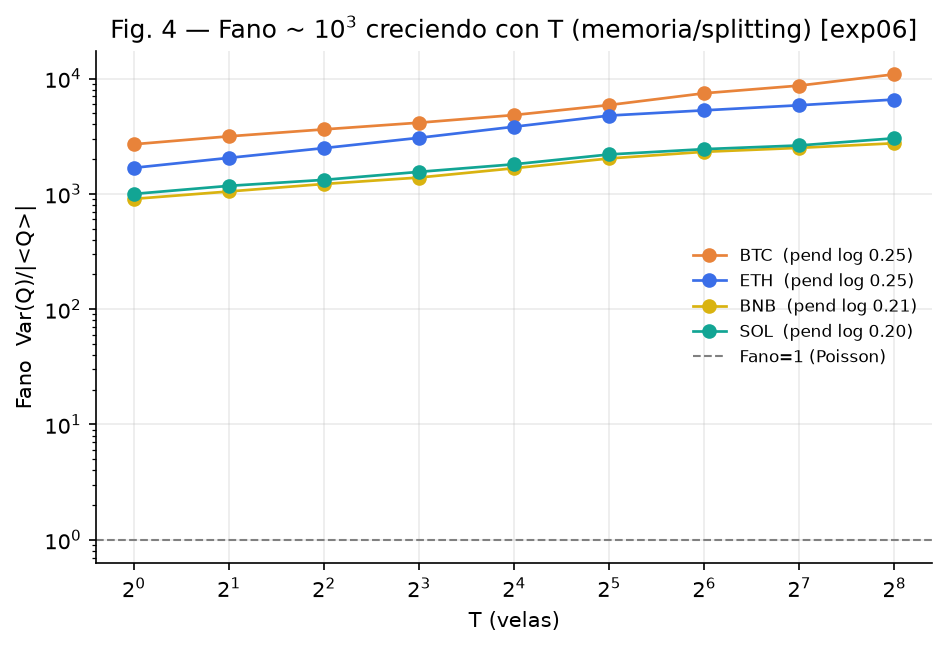
\includegraphics[width=\columnwidth]{../output/figuras/fig4_fano.png}
  \caption{Fano factor of the transferred signed flow against counting window,
  hourly data. The level is of order $10^{3}$ and grows with $T$. A free-fermion
  counting problem is bounded below the dashed Poisson line, and the explicit
  device calculation described in the text returns $\mathcal{F}=0.33$.}
  \label{fig:fano}
\end{figure}

\paragraph*{A crossover prediction, and its test.}
The second departure is more specific, and it is predictive. For a single
power-law kernel $C_\eps(\tau)=A\tau^{-a}$ with $0<a<1$,
\begin{equation}
  V_T=\!\!\sum_{t,t'=1}^{T}\!\!C_\eps(t-t')
     \simeq\frac{2A}{(1-a)(2-a)}\,T^{\,2-a} ,
  \label{eq:varscaling}
\end{equation}
so the counting variance grows with exponent $\nu=2-a$ set by the correlation
decay. The measured $C_\eps$, however, is not a single power law: fitting local
slopes separately gives a fast regime $a_f$ over $\tau\in[2,10]$ and a slow one
$a_s$ over $\tau\in[10,50]$, with $a_f>a_s$ in all four assets, and removing the
daily seasonal component leaves both essentially unchanged. For the reference
asset, $a_f=1.00\pm0.15$ and $a_s=0.17\pm0.13$.

Equation~\eqref{eq:varscaling} then cannot hold with a single $\nu$. Short
windows sample the fast regime and long windows the slow one, so the
\emph{local} logarithmic slope must drift,
\begin{equation}
  \nu_{\rm loc}(T):\;2-a_f\;\longrightarrow\;2-a_s ,
  \label{eq:crossover}
\end{equation}
here a band $[1.00,1.83]$.

The prediction has no free parameters and crosses observable families: $a_f$ and
$a_s$ are measured in the correlation sector, $\nu$ in the counting sector, so
the test cannot be circular. It is confirmed. The measured exponent lies inside
the predicted band, and exceeds unity in every asset:
$\nu=1.31$--$1.43$ from the block variance and $1.10$--$1.36$ from three
estimators built to be insensitive to the mean (below), against $\nu=1$ for the
free-fermion device and $[0.90,1.14]$ for a permutation null that preserves the
marginal distribution and destroys memory. Superdiffusive growth of the
counting variance is a statement about memory alone, and it is what the
correlation sector demands.

The apparent \emph{drift} of the local exponent, however, is not identified,
and we flag it rather than claim it. $V_T$ is a sample variance over
non-overlapping blocks, so a drift in the per-block mean enters it with a term
growing as $T^2$ --- steeper than the kernel allows and biased the same way. The
flow does drift: it carries a persistent sell-side bias and modulates with the
daily cycle. The Haar difference between adjacent blocks separates the two,
since $\Var(Q_T^{(2)}-Q_T^{(1)})=4V_T-V_{2T}=A(4-2^{\nu})T^{\nu}$ carries the
same exponent with a constant mean cancelled exactly, and filters with more
vanishing moments remove linear and quadratic drifts as well
\cite{daubechies1992}. All four estimators agree to $0.01$ on synthetic series
of known $\nu$, and the injected drift moves only the block one --- so the
comparison has the required sensitivity. On the data the block estimator is the
highest of the four in every asset, by $0.13$ to $0.29$; injecting each asset's
own measured drift onto a clean synthetic series reproduces up to $0.13$ of
that gap, and removing the drift by hand closes it. The drift-blind estimators
neither reproduce the crossover nor exclude it, their local slopes carrying
errors of $\pm0.05$ to $\pm0.22$ against a claimed excursion of $0.28$. We
therefore report Eq.~\eqref{eq:crossover} as consistent with the data and not
discriminated by them, and make no inference from it against a one-component
bath.

A corollary of Eq.~\eqref{eq:identity} combined with
Eq.~\eqref{eq:varscaling} is that the affinity must dilute with scale as
$A_T\propto T^{a-1}$; the parameter-free form $A_{T_2}/A_{T_1} =
(T_2/T_1)(V_{T_1}/V_{T_2})$ reproduces the measured ratio to within $0.5$--$13\%$
for the two assets whose affinity is stable across the sample, and fails badly
for the two whose affinity sits at the noise level --- failing, that is,
precisely where the predicted quantity is not determined.

\begin{figure}[t]
  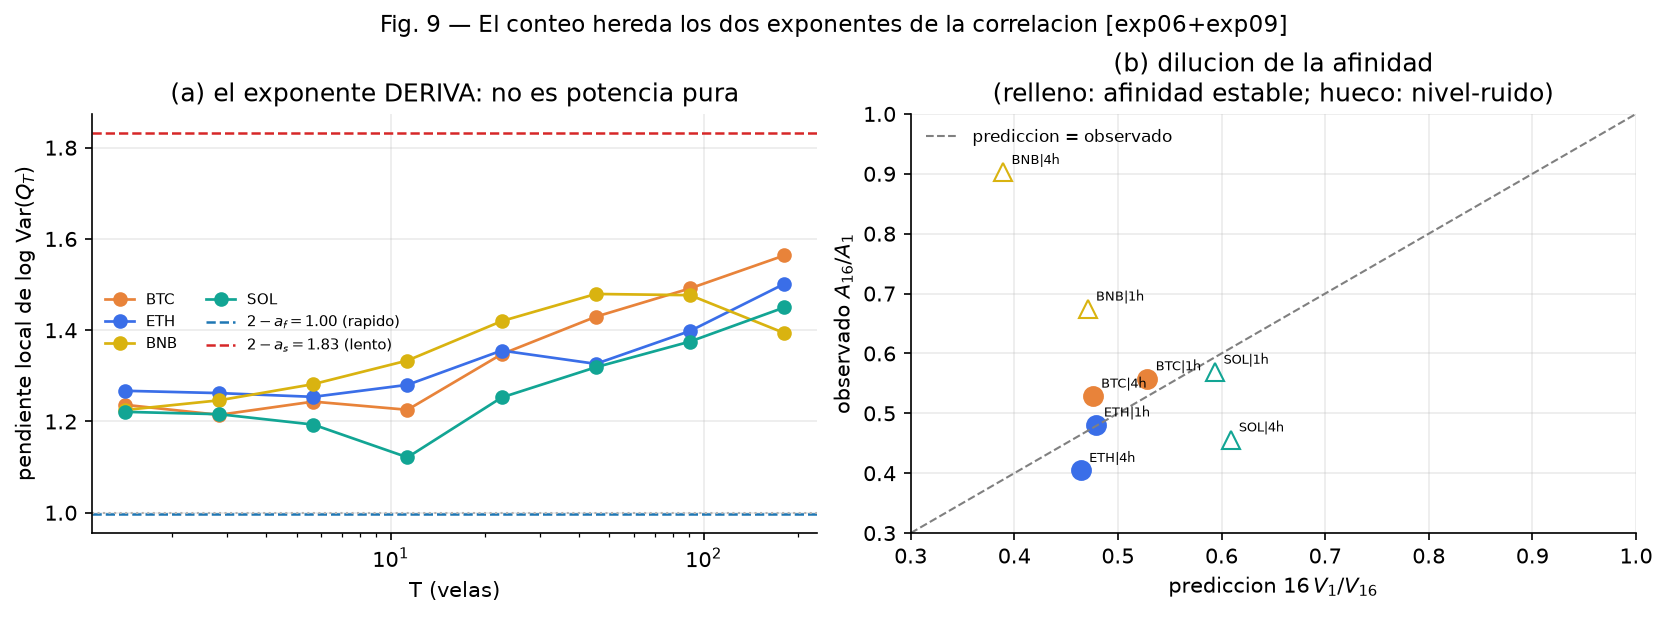
\includegraphics[width=\columnwidth]{../output/figuras/fig9_crossover_exponente.png}
  \caption{Test of Eq.~\eqref{eq:varscaling}. (a) The local logarithmic slope
  of the block counting variance against window size, in all four assets,
  within the band set by the two correlation exponents measured independently.
  The band is the confirmed prediction; the upward drift within it is not
  identified, since a drifting mean inflates this estimator and drift-blind
  estimators do not reproduce the drift (text). (b) The parameter-free
  affinity dilution against the measured ratio; filled symbols mark assets with
  a stable affinity, open symbols those at the noise level.}
  \label{fig:crossover}
\end{figure}

\paragraph*{Discussion.}
Three statements, in the order in which they constrain each other. The
second-order counting sector of order flow is closed and empty: its fluctuation
symmetry is an identity, and its variance is the autocorrelation. The counting
sector beyond second order is not empty and is not reachable by free transport,
by margins that are set by statistics rather than by parameters. And the memory
that produces the excess is two-component, in a way that makes a falsifiable and
parameter-free prediction about the counting variance which the data confirm.

We would emphasise the methodological point alongside the physical one. The
appeal of a fluctuation-theorem reading of markets is that a log-ratio of
forward and reversed distributions is easy to measure and lands on a clean
straight line. Equation~\eqref{eq:identity} says that the straight line is
guaranteed for any Gaussian observable, so its appearance is not a discovery,
and the slope is not an independent parameter. As statistical-physics
descriptions of markets continue to be developed, we think this distinction is
worth having explicitly, because the informative content lives entirely on the
other side of it --- in the Fano factor, in the higher cumulants, and in the
scale dependence of the memory.

\begin{acknowledgments}
\end{acknowledgments}

\bibliography{refs}

\end{document}
